\documentclass[twoside]{book}

% Packages required by doxygen
\usepackage{fixltx2e}
\usepackage{calc}
\usepackage{doxygen}
\usepackage{graphicx}
\usepackage[utf8]{inputenc}
\usepackage{makeidx}
\usepackage{multicol}
\usepackage{multirow}
\PassOptionsToPackage{warn}{textcomp}
\usepackage{textcomp}
\usepackage[nointegrals]{wasysym}
\usepackage[table]{xcolor}

% Font selection
\usepackage[T1]{fontenc}
\usepackage[scaled=.90]{helvet}
\usepackage{courier}
\usepackage{amssymb}
\usepackage{sectsty}
\renewcommand{\familydefault}{\sfdefault}
\allsectionsfont{%
  \fontseries{bc}\selectfont%
  \color{darkgray}%
}
\renewcommand{\DoxyLabelFont}{%
  \fontseries{bc}\selectfont%
  \color{darkgray}%
}
\newcommand{\+}{\discretionary{\mbox{\scriptsize$\hookleftarrow$}}{}{}}

% Page & text layout
\usepackage{geometry}
\geometry{%
  a4paper,%
  top=2.5cm,%
  bottom=2.5cm,%
  left=2.5cm,%
  right=2.5cm%
}
\tolerance=750
\hfuzz=15pt
\hbadness=750
\setlength{\emergencystretch}{15pt}
\setlength{\parindent}{0cm}
\setlength{\parskip}{0.2cm}
\makeatletter
\renewcommand{\paragraph}{%
  \@startsection{paragraph}{4}{0ex}{-1.0ex}{1.0ex}{%
    \normalfont\normalsize\bfseries\SS@parafont%
  }%
}
\renewcommand{\subparagraph}{%
  \@startsection{subparagraph}{5}{0ex}{-1.0ex}{1.0ex}{%
    \normalfont\normalsize\bfseries\SS@subparafont%
  }%
}
\makeatother

% Headers & footers
\usepackage{fancyhdr}
\pagestyle{fancyplain}
\fancyhead[LE]{\fancyplain{}{\bfseries\thepage}}
\fancyhead[CE]{\fancyplain{}{}}
\fancyhead[RE]{\fancyplain{}{\bfseries\leftmark}}
\fancyhead[LO]{\fancyplain{}{\bfseries\rightmark}}
\fancyhead[CO]{\fancyplain{}{}}
\fancyhead[RO]{\fancyplain{}{\bfseries\thepage}}
\fancyfoot[LE]{\fancyplain{}{}}
\fancyfoot[CE]{\fancyplain{}{}}
\fancyfoot[RE]{\fancyplain{}{\bfseries\scriptsize Generated on Mon Nov 17 2014 09\+:25\+:24 for P2\+P\+Encrypted\+Tkinter\+App by Doxygen }}
\fancyfoot[LO]{\fancyplain{}{\bfseries\scriptsize Generated on Mon Nov 17 2014 09\+:25\+:24 for P2\+P\+Encrypted\+Tkinter\+App by Doxygen }}
\fancyfoot[CO]{\fancyplain{}{}}
\fancyfoot[RO]{\fancyplain{}{}}
\renewcommand{\footrulewidth}{0.4pt}
\renewcommand{\chaptermark}[1]{%
  \markboth{#1}{}%
}
\renewcommand{\sectionmark}[1]{%
  \markright{\thesection\ #1}%
}

% Indices & bibliography
\usepackage{natbib}
\usepackage[titles]{tocloft}
\setcounter{tocdepth}{3}
\setcounter{secnumdepth}{5}
\makeindex

% Hyperlinks (required, but should be loaded last)
\usepackage{ifpdf}
\ifpdf
  \usepackage[pdftex,pagebackref=true]{hyperref}
\else
  \usepackage[ps2pdf,pagebackref=true]{hyperref}
\fi
\hypersetup{%
  colorlinks=true,%
  linkcolor=blue,%
  citecolor=blue,%
  unicode%
}

% Custom commands
\newcommand{\clearemptydoublepage}{%
  \newpage{\pagestyle{empty}\cleardoublepage}%
}


%===== C O N T E N T S =====

\begin{document}

% Titlepage & ToC
\hypersetup{pageanchor=false,
             bookmarks=true,
             bookmarksnumbered=true,
             pdfencoding=unicode
            }
\pagenumbering{roman}
\begin{titlepage}
\vspace*{7cm}
\begin{center}%
{\Large P2\+P\+Encrypted\+Tkinter\+App }\\
\vspace*{1cm}
{\large Generated by Doxygen 1.8.8}\\
\vspace*{0.5cm}
{\small Mon Nov 17 2014 09:25:24}\\
\end{center}
\end{titlepage}
\clearemptydoublepage
\tableofcontents
\clearemptydoublepage
\pagenumbering{arabic}
\hypersetup{pageanchor=true}

%--- Begin generated contents ---
\chapter{Namespace Index}
\section{Packages}
Here are the packages with brief descriptions (if available)\+:\begin{DoxyCompactList}
\item\contentsline{section}{\hyperlink{namespacegui_version}{gui\+Version} }{\pageref{namespacegui_version}}{}
\item\contentsline{section}{\hyperlink{namespacenew_server}{new\+Server} }{\pageref{namespacenew_server}}{}
\end{DoxyCompactList}

\chapter{Hierarchical Index}
\section{Class Hierarchy}
This inheritance list is sorted roughly, but not completely, alphabetically\+:\begin{DoxyCompactList}
\item \contentsline{section}{gui\+Version.\+F}{\pageref{classgui_version_1_1_f}}{}
\item \contentsline{section}{new\+Server.\+F}{\pageref{classnew_server_1_1_f}}{}
\item \contentsline{section}{Frame}{\pageref{class_frame}}{}
\begin{DoxyCompactList}
\item \contentsline{section}{gui\+Version.\+Chat\+Client\+G\+U\+I}{\pageref{classgui_version_1_1_chat_client_g_u_i}}{}
\end{DoxyCompactList}
\end{DoxyCompactList}

\chapter{Class Index}
\section{Class List}
Here are the classes, structs, unions and interfaces with brief descriptions\+:\begin{DoxyCompactList}
\item\contentsline{section}{\hyperlink{classgui_version_1_1_chat_client_g_u_i}{gui\+Version.\+Chat\+Client\+G\+U\+I} }{\pageref{classgui_version_1_1_chat_client_g_u_i}}{}
\item\contentsline{section}{\hyperlink{classgui_version_1_1_f}{gui\+Version.\+F} }{\pageref{classgui_version_1_1_f}}{}
\item\contentsline{section}{\hyperlink{classnew_server_1_1_f}{new\+Server.\+F} }{\pageref{classnew_server_1_1_f}}{}
\item\contentsline{section}{\hyperlink{class_frame}{Frame} }{\pageref{class_frame}}{}
\end{DoxyCompactList}

\chapter{File Index}
\section{File List}
Here is a list of all files with brief descriptions\+:\begin{DoxyCompactList}
\item\contentsline{section}{\hyperlink{gui_version_8py}{gui\+Version.\+py} }{\pageref{gui_version_8py}}{}
\item\contentsline{section}{\hyperlink{new_server_8py}{new\+Server.\+py} }{\pageref{new_server_8py}}{}
\end{DoxyCompactList}

\chapter{Namespace Documentation}
\hypertarget{namespacegui_version}{}\section{gui\+Version Namespace Reference}
\label{namespacegui_version}\index{gui\+Version@{gui\+Version}}
\subsection*{Classes}
\begin{DoxyCompactItemize}
\item 
class \hyperlink{classgui_version_1_1_chat_client_g_u_i}{Chat\+Client\+G\+U\+I}
\begin{DoxyCompactList}\small\item\em The Main class has all the methods used by the gui. \end{DoxyCompactList}\item 
class \hyperlink{classgui_version_1_1_f}{F}
\begin{DoxyCompactList}\small\item\em Monkey Patch stdout so the print statement has the timestamp appended to it. \end{DoxyCompactList}\end{DoxyCompactItemize}
\subsection*{Functions}
\begin{DoxyCompactItemize}
\item 
def \hyperlink{namespacegui_version_ae8a9c77879e18f58a45597b28e21042b}{zip\+\_\+and\+\_\+encrypt\+\_\+val} (clear\+\_\+text, key)
\begin{DoxyCompactList}\small\item\em Function that encrypts your string. \end{DoxyCompactList}\item 
def \hyperlink{namespacegui_version_a2925a99a40df97be6ae16f1a22184b24}{decrypt\+\_\+val\+\_\+and\+\_\+unzip} (cipher\+\_\+text, key)
\begin{DoxyCompactList}\small\item\em Function that decrypts an encypted string. \end{DoxyCompactList}\item 
def \hyperlink{namespacegui_version_a79d3b927a5ac9c40a255afc12ebfa5bb}{main} ()
\end{DoxyCompactItemize}
\subsection*{Variables}
\begin{DoxyCompactItemize}
\item 
tuple \hyperlink{namespacegui_version_ad80b491a9fbc91c221e73a124bff5d05}{M\+A\+S\+T\+E\+R\+\_\+\+K\+E\+Y} = hashlib.\+sha256(\char`\"{}Some-\/long-\/base-\/key-\/to-\/use-\/as-\/encyrption-\/key\char`\"{})
\begin{DoxyCompactList}\small\item\em somethings wrong when the K\+E\+Y I\+S 256bytes so im hasing it into a 256 byte string \end{DoxyCompactList}\item 
\hyperlink{namespacegui_version_a77c635f5f5d51002c89931af7228063c}{old\+\_\+f} = sys.\+stdout
\begin{DoxyCompactList}\small\item\em Keep a reference of the old stdout. \end{DoxyCompactList}\end{DoxyCompactItemize}


\subsection{Function Documentation}
\hypertarget{namespacegui_version_a2925a99a40df97be6ae16f1a22184b24}{}\index{gui\+Version@{gui\+Version}!decrypt\+\_\+val\+\_\+and\+\_\+unzip@{decrypt\+\_\+val\+\_\+and\+\_\+unzip}}
\index{decrypt\+\_\+val\+\_\+and\+\_\+unzip@{decrypt\+\_\+val\+\_\+and\+\_\+unzip}!gui\+Version@{gui\+Version}}
\subsubsection[{decrypt\+\_\+val\+\_\+and\+\_\+unzip}]{\setlength{\rightskip}{0pt plus 5cm}def gui\+Version.\+decrypt\+\_\+val\+\_\+and\+\_\+unzip (
\begin{DoxyParamCaption}
\item[{}]{cipher\+\_\+text, }
\item[{}]{key}
\end{DoxyParamCaption}
)}\label{namespacegui_version_a2925a99a40df97be6ae16f1a22184b24}


Function that decrypts an encypted string. 

it doesnt decompress it.. caused errors 
\begin{DoxyParams}{Parameters}
{\em clear\+\_\+text} & The unencypted text that you want to encrypt \\
\hline
{\em key} & The key you want to encrypt the clear text with \\
\hline
\end{DoxyParams}


Definition at line 39 of file gui\+Version.\+py.

\hypertarget{namespacegui_version_a79d3b927a5ac9c40a255afc12ebfa5bb}{}\index{gui\+Version@{gui\+Version}!main@{main}}
\index{main@{main}!gui\+Version@{gui\+Version}}
\subsubsection[{main}]{\setlength{\rightskip}{0pt plus 5cm}def gui\+Version.\+main (
\begin{DoxyParamCaption}
{}
\end{DoxyParamCaption}
)}\label{namespacegui_version_a79d3b927a5ac9c40a255afc12ebfa5bb}


Definition at line 254 of file gui\+Version.\+py.

\hypertarget{namespacegui_version_ae8a9c77879e18f58a45597b28e21042b}{}\index{gui\+Version@{gui\+Version}!zip\+\_\+and\+\_\+encrypt\+\_\+val@{zip\+\_\+and\+\_\+encrypt\+\_\+val}}
\index{zip\+\_\+and\+\_\+encrypt\+\_\+val@{zip\+\_\+and\+\_\+encrypt\+\_\+val}!gui\+Version@{gui\+Version}}
\subsubsection[{zip\+\_\+and\+\_\+encrypt\+\_\+val}]{\setlength{\rightskip}{0pt plus 5cm}def gui\+Version.\+zip\+\_\+and\+\_\+encrypt\+\_\+val (
\begin{DoxyParamCaption}
\item[{}]{clear\+\_\+text, }
\item[{}]{key}
\end{DoxyParamCaption}
)}\label{namespacegui_version_ae8a9c77879e18f58a45597b28e21042b}


Function that encrypts your string. 

it doesnt compress it since i had errors decompressing 
\begin{DoxyParams}{Parameters}
{\em clear\+\_\+text} & The unencypted text that you want to encrypt \\
\hline
{\em key} & The key you want to encrypt the clear text with \\
\hline
\end{DoxyParams}


Definition at line 27 of file gui\+Version.\+py.



\subsection{Variable Documentation}
\hypertarget{namespacegui_version_ad80b491a9fbc91c221e73a124bff5d05}{}\index{gui\+Version@{gui\+Version}!M\+A\+S\+T\+E\+R\+\_\+\+K\+E\+Y@{M\+A\+S\+T\+E\+R\+\_\+\+K\+E\+Y}}
\index{M\+A\+S\+T\+E\+R\+\_\+\+K\+E\+Y@{M\+A\+S\+T\+E\+R\+\_\+\+K\+E\+Y}!gui\+Version@{gui\+Version}}
\subsubsection[{M\+A\+S\+T\+E\+R\+\_\+\+K\+E\+Y}]{\setlength{\rightskip}{0pt plus 5cm}tuple gui\+Version.\+M\+A\+S\+T\+E\+R\+\_\+\+K\+E\+Y = hashlib.\+sha256(\char`\"{}Some-\/long-\/base-\/key-\/to-\/use-\/as-\/encyrption-\/key\char`\"{})}\label{namespacegui_version_ad80b491a9fbc91c221e73a124bff5d05}


somethings wrong when the K\+E\+Y I\+S 256bytes so im hasing it into a 256 byte string 



Definition at line 11 of file gui\+Version.\+py.

\hypertarget{namespacegui_version_a77c635f5f5d51002c89931af7228063c}{}\index{gui\+Version@{gui\+Version}!old\+\_\+f@{old\+\_\+f}}
\index{old\+\_\+f@{old\+\_\+f}!gui\+Version@{gui\+Version}}
\subsubsection[{old\+\_\+f}]{\setlength{\rightskip}{0pt plus 5cm}gui\+Version.\+old\+\_\+f = sys.\+stdout}\label{namespacegui_version_a77c635f5f5d51002c89931af7228063c}


Keep a reference of the old stdout. 



Definition at line 13 of file gui\+Version.\+py.


\hypertarget{namespacenew_server}{}\section{new\+Server Namespace Reference}
\label{namespacenew_server}\index{new\+Server@{new\+Server}}
\subsection*{Classes}
\begin{DoxyCompactItemize}
\item 
class \hyperlink{classnew_server_1_1_f}{F}
\end{DoxyCompactItemize}
\subsection*{Functions}
\begin{DoxyCompactItemize}
\item 
def \hyperlink{namespacenew_server_ae9d433fa51d0c682b18c3b9879cb0a1f}{process\+Client\+Commands} (cmd, client\+Socket)
\item 
def \hyperlink{namespacenew_server_a35090b3a9dc30b6f28f73efc7e104cc9}{send\+Response\+From\+Server} (response, user\+Socket)
\item 
def \hyperlink{namespacenew_server_af9cb120a81a10188d82dd3aaec0eea2d}{client\+Message} (client\+Soc, client\+Addr, server\+Socket)
\item 
def \hyperlink{namespacenew_server_a32d38e8c1989792b3d964150ed181779}{broadcast} (server\+\_\+socket, sock, message)
\item 
def \hyperlink{namespacenew_server_abe65059086c03efc53e029abe9cc98fc}{chat\+\_\+server} (host, port)
\end{DoxyCompactItemize}
\subsection*{Variables}
\begin{DoxyCompactItemize}
\item 
list \hyperlink{namespacenew_server_a85c087d4ca25a1782111a4dca1169b6d}{P\+O\+S\+S\+I\+B\+L\+E\+\_\+\+C\+O\+M\+M\+A\+N\+D\+S} = \mbox{[}\char`\"{}join\char`\"{},\char`\"{}bye\char`\"{},\char`\"{}crea\char`\"{},\char`\"{}subs\char`\"{},\char`\"{}unsu\char`\"{},\char`\"{}defa\char`\"{},\char`\"{}lscr\char`\"{},\char`\"{}lssu\char`\"{},\char`\"{}read\char`\"{},\char`\"{}writ\char`\"{},\char`\"{}chmod\char`\"{}\mbox{]}
\item 
string \hyperlink{namespacenew_server_a6c675879b0fb0559c66f1bf7118300fd}{H\+O\+S\+T} = '0.\+0.\+0.\+0'
\item 
list \hyperlink{namespacenew_server_a0472f2f3fb3afb95020b3c9ea29c0af4}{S\+O\+C\+K\+E\+T\+\_\+\+L\+I\+S\+T} = \mbox{[}$\,$\mbox{]}
\item 
int \hyperlink{namespacenew_server_a7d87ef1942af615eeec258c226e5b859}{R\+E\+C\+V\+\_\+\+B\+U\+F\+F\+E\+R} = 4096
\item 
int \hyperlink{namespacenew_server_a10c03320240322f838e9f19a686e825d}{P\+O\+R\+T} = 8022
\item 
\hyperlink{namespacenew_server_a771dfc755950f86e03d334f4d04dc59e}{old\+\_\+f} = sys.\+stdout
\end{DoxyCompactItemize}


\subsection{Function Documentation}
\hypertarget{namespacenew_server_a32d38e8c1989792b3d964150ed181779}{}\index{new\+Server@{new\+Server}!broadcast@{broadcast}}
\index{broadcast@{broadcast}!new\+Server@{new\+Server}}
\subsubsection[{broadcast}]{\setlength{\rightskip}{0pt plus 5cm}def new\+Server.\+broadcast (
\begin{DoxyParamCaption}
\item[{}]{server\+\_\+socket, }
\item[{}]{sock, }
\item[{}]{message}
\end{DoxyParamCaption}
)}\label{namespacenew_server_a32d38e8c1989792b3d964150ed181779}


Definition at line 56 of file new\+Server.\+py.

\hypertarget{namespacenew_server_abe65059086c03efc53e029abe9cc98fc}{}\index{new\+Server@{new\+Server}!chat\+\_\+server@{chat\+\_\+server}}
\index{chat\+\_\+server@{chat\+\_\+server}!new\+Server@{new\+Server}}
\subsubsection[{chat\+\_\+server}]{\setlength{\rightskip}{0pt plus 5cm}def new\+Server.\+chat\+\_\+server (
\begin{DoxyParamCaption}
\item[{}]{host, }
\item[{}]{port}
\end{DoxyParamCaption}
)}\label{namespacenew_server_abe65059086c03efc53e029abe9cc98fc}


Definition at line 70 of file new\+Server.\+py.

\hypertarget{namespacenew_server_af9cb120a81a10188d82dd3aaec0eea2d}{}\index{new\+Server@{new\+Server}!client\+Message@{client\+Message}}
\index{client\+Message@{client\+Message}!new\+Server@{new\+Server}}
\subsubsection[{client\+Message}]{\setlength{\rightskip}{0pt plus 5cm}def new\+Server.\+client\+Message (
\begin{DoxyParamCaption}
\item[{}]{client\+Soc, }
\item[{}]{client\+Addr, }
\item[{}]{server\+Socket}
\end{DoxyParamCaption}
)}\label{namespacenew_server_af9cb120a81a10188d82dd3aaec0eea2d}


Definition at line 36 of file new\+Server.\+py.

\hypertarget{namespacenew_server_ae9d433fa51d0c682b18c3b9879cb0a1f}{}\index{new\+Server@{new\+Server}!process\+Client\+Commands@{process\+Client\+Commands}}
\index{process\+Client\+Commands@{process\+Client\+Commands}!new\+Server@{new\+Server}}
\subsubsection[{process\+Client\+Commands}]{\setlength{\rightskip}{0pt plus 5cm}def new\+Server.\+process\+Client\+Commands (
\begin{DoxyParamCaption}
\item[{}]{cmd, }
\item[{}]{client\+Socket}
\end{DoxyParamCaption}
)}\label{namespacenew_server_ae9d433fa51d0c682b18c3b9879cb0a1f}


Definition at line 23 of file new\+Server.\+py.

\hypertarget{namespacenew_server_a35090b3a9dc30b6f28f73efc7e104cc9}{}\index{new\+Server@{new\+Server}!send\+Response\+From\+Server@{send\+Response\+From\+Server}}
\index{send\+Response\+From\+Server@{send\+Response\+From\+Server}!new\+Server@{new\+Server}}
\subsubsection[{send\+Response\+From\+Server}]{\setlength{\rightskip}{0pt plus 5cm}def new\+Server.\+send\+Response\+From\+Server (
\begin{DoxyParamCaption}
\item[{}]{response, }
\item[{}]{user\+Socket}
\end{DoxyParamCaption}
)}\label{namespacenew_server_a35090b3a9dc30b6f28f73efc7e104cc9}


Definition at line 33 of file new\+Server.\+py.



\subsection{Variable Documentation}
\hypertarget{namespacenew_server_a6c675879b0fb0559c66f1bf7118300fd}{}\index{new\+Server@{new\+Server}!H\+O\+S\+T@{H\+O\+S\+T}}
\index{H\+O\+S\+T@{H\+O\+S\+T}!new\+Server@{new\+Server}}
\subsubsection[{H\+O\+S\+T}]{\setlength{\rightskip}{0pt plus 5cm}string new\+Server.\+H\+O\+S\+T = '0.\+0.\+0.\+0'}\label{namespacenew_server_a6c675879b0fb0559c66f1bf7118300fd}


Definition at line 9 of file new\+Server.\+py.

\hypertarget{namespacenew_server_a771dfc755950f86e03d334f4d04dc59e}{}\index{new\+Server@{new\+Server}!old\+\_\+f@{old\+\_\+f}}
\index{old\+\_\+f@{old\+\_\+f}!new\+Server@{new\+Server}}
\subsubsection[{old\+\_\+f}]{\setlength{\rightskip}{0pt plus 5cm}new\+Server.\+old\+\_\+f = sys.\+stdout}\label{namespacenew_server_a771dfc755950f86e03d334f4d04dc59e}


Definition at line 17 of file new\+Server.\+py.

\hypertarget{namespacenew_server_a10c03320240322f838e9f19a686e825d}{}\index{new\+Server@{new\+Server}!P\+O\+R\+T@{P\+O\+R\+T}}
\index{P\+O\+R\+T@{P\+O\+R\+T}!new\+Server@{new\+Server}}
\subsubsection[{P\+O\+R\+T}]{\setlength{\rightskip}{0pt plus 5cm}int new\+Server.\+P\+O\+R\+T = 8022}\label{namespacenew_server_a10c03320240322f838e9f19a686e825d}


Definition at line 14 of file new\+Server.\+py.

\hypertarget{namespacenew_server_a85c087d4ca25a1782111a4dca1169b6d}{}\index{new\+Server@{new\+Server}!P\+O\+S\+S\+I\+B\+L\+E\+\_\+\+C\+O\+M\+M\+A\+N\+D\+S@{P\+O\+S\+S\+I\+B\+L\+E\+\_\+\+C\+O\+M\+M\+A\+N\+D\+S}}
\index{P\+O\+S\+S\+I\+B\+L\+E\+\_\+\+C\+O\+M\+M\+A\+N\+D\+S@{P\+O\+S\+S\+I\+B\+L\+E\+\_\+\+C\+O\+M\+M\+A\+N\+D\+S}!new\+Server@{new\+Server}}
\subsubsection[{P\+O\+S\+S\+I\+B\+L\+E\+\_\+\+C\+O\+M\+M\+A\+N\+D\+S}]{\setlength{\rightskip}{0pt plus 5cm}list new\+Server.\+P\+O\+S\+S\+I\+B\+L\+E\+\_\+\+C\+O\+M\+M\+A\+N\+D\+S = \mbox{[}\char`\"{}join\char`\"{},\char`\"{}bye\char`\"{},\char`\"{}crea\char`\"{},\char`\"{}subs\char`\"{},\char`\"{}unsu\char`\"{},\char`\"{}defa\char`\"{},\char`\"{}lscr\char`\"{},\char`\"{}lssu\char`\"{},\char`\"{}read\char`\"{},\char`\"{}writ\char`\"{},\char`\"{}chmod\char`\"{}\mbox{]}}\label{namespacenew_server_a85c087d4ca25a1782111a4dca1169b6d}


Definition at line 7 of file new\+Server.\+py.

\hypertarget{namespacenew_server_a7d87ef1942af615eeec258c226e5b859}{}\index{new\+Server@{new\+Server}!R\+E\+C\+V\+\_\+\+B\+U\+F\+F\+E\+R@{R\+E\+C\+V\+\_\+\+B\+U\+F\+F\+E\+R}}
\index{R\+E\+C\+V\+\_\+\+B\+U\+F\+F\+E\+R@{R\+E\+C\+V\+\_\+\+B\+U\+F\+F\+E\+R}!new\+Server@{new\+Server}}
\subsubsection[{R\+E\+C\+V\+\_\+\+B\+U\+F\+F\+E\+R}]{\setlength{\rightskip}{0pt plus 5cm}int new\+Server.\+R\+E\+C\+V\+\_\+\+B\+U\+F\+F\+E\+R = 4096}\label{namespacenew_server_a7d87ef1942af615eeec258c226e5b859}


Definition at line 13 of file new\+Server.\+py.

\hypertarget{namespacenew_server_a0472f2f3fb3afb95020b3c9ea29c0af4}{}\index{new\+Server@{new\+Server}!S\+O\+C\+K\+E\+T\+\_\+\+L\+I\+S\+T@{S\+O\+C\+K\+E\+T\+\_\+\+L\+I\+S\+T}}
\index{S\+O\+C\+K\+E\+T\+\_\+\+L\+I\+S\+T@{S\+O\+C\+K\+E\+T\+\_\+\+L\+I\+S\+T}!new\+Server@{new\+Server}}
\subsubsection[{S\+O\+C\+K\+E\+T\+\_\+\+L\+I\+S\+T}]{\setlength{\rightskip}{0pt plus 5cm}list new\+Server.\+S\+O\+C\+K\+E\+T\+\_\+\+L\+I\+S\+T = \mbox{[}$\,$\mbox{]}}\label{namespacenew_server_a0472f2f3fb3afb95020b3c9ea29c0af4}


Definition at line 12 of file new\+Server.\+py.


\chapter{Class Documentation}
\hypertarget{classgui_version_1_1_chat_client_g_u_i}{}\section{gui\+Version.\+Chat\+Client\+G\+U\+I Class Reference}
\label{classgui_version_1_1_chat_client_g_u_i}\index{gui\+Version.\+Chat\+Client\+G\+U\+I@{gui\+Version.\+Chat\+Client\+G\+U\+I}}


The Main class has all the methods used by the gui.  


Inheritance diagram for gui\+Version.\+Chat\+Client\+G\+U\+I\+:\begin{figure}[H]
\begin{center}
\leavevmode
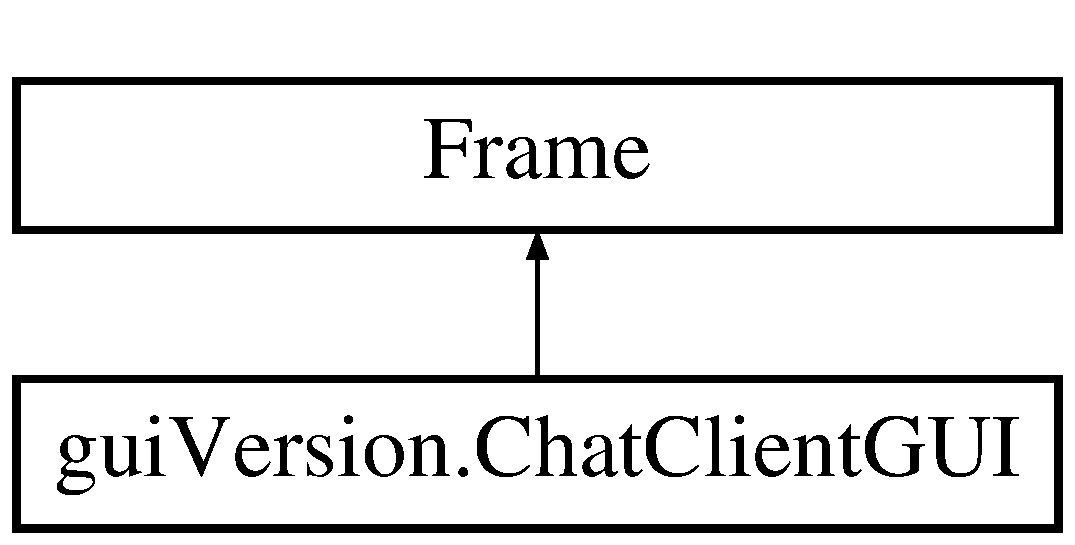
\includegraphics[height=2.000000cm]{classgui_version_1_1_chat_client_g_u_i}
\end{center}
\end{figure}
\subsection*{Public Member Functions}
\begin{DoxyCompactItemize}
\item 
def \hyperlink{classgui_version_1_1_chat_client_g_u_i_ae6788c5b8f15cd3ac7a844cee72e06a3}{\+\_\+\+\_\+init\+\_\+\+\_\+} (self)
\item 
def \hyperlink{classgui_version_1_1_chat_client_g_u_i_a768dd49f34840a662bc12636dcb8f18a}{chat\+Room\+Window\+Init} (self)
\begin{DoxyCompactList}\small\item\em Creates the textbox that the messages go into. \end{DoxyCompactList}\item 
def \hyperlink{classgui_version_1_1_chat_client_g_u_i_a1788a126553ae97447343bd9f4187624}{chat\+Room\+Text\+Box\+Init} (self)
\begin{DoxyCompactList}\small\item\em Create the entry widget that user types messages into. \end{DoxyCompactList}\item 
def \hyperlink{classgui_version_1_1_chat_client_g_u_i_ad5e98841e008476eee6015e5b8bf6eee}{send\+Button\+Init} (self)
\begin{DoxyCompactList}\small\item\em Creates the send button that sends the message The meesage is also binded to send with the pressing of the return key. \end{DoxyCompactList}\item 
def \hyperlink{classgui_version_1_1_chat_client_g_u_i_a16414e83201878b6a1565fdf0600f15a}{encryption\+Key\+Init} (self)
\begin{DoxyCompactList}\small\item\em Create the entry widget that user types their encryption key into. \end{DoxyCompactList}\item 
def \hyperlink{classgui_version_1_1_chat_client_g_u_i_acb99a090317b6806b24e91ef4ac4b0e2}{icon\+Init} (self)
\item 
def \hyperlink{classgui_version_1_1_chat_client_g_u_i_ac68b416d5a4d4962b76752f1aa78bccb}{highlight} (self, args)
\begin{DoxyCompactList}\small\item\em Searches text box for the regex provided and highlight all matches to have blue text We can end up using this for more than just highlighting the user messages. \end{DoxyCompactList}\item 
def \hyperlink{classgui_version_1_1_chat_client_g_u_i_ad0b24322eeb5217d9410ee68fb054d42}{set\+Key} (self, secret\+Key)
\begin{DoxyCompactList}\small\item\em Set the users secret key, change image based on key,. \end{DoxyCompactList}\item 
def \hyperlink{classgui_version_1_1_chat_client_g_u_i_a976bddea0e9e23dd9e2245aa002a354f}{connect\+To\+Server} (self)
\item 
def \hyperlink{classgui_version_1_1_chat_client_g_u_i_a8de44a4f22866fe79ee14d0536120fa4}{get\+Message\+Thread} (self, \hyperlink{classgui_version_1_1_chat_client_g_u_i_ad0d119fff1856994d498e1e9861451d5}{client\+Socket}, host)
\begin{DoxyCompactList}\small\item\em This is where the magic happens a thread reads from the specified port constantly if there is data it continues by processing it, (decrypt, strip padding, catch errors The danger here is I am modifying the app from a thread that is not the main thread. \end{DoxyCompactList}\item 
def \hyperlink{classgui_version_1_1_chat_client_g_u_i_afbeef14d848917e111de1d91e325662c}{process\+Send\+Button} (self, args)
\begin{DoxyCompactList}\small\item\em Gets called on enter press or send button This is where we decide to compress the cmds sent to server. \end{DoxyCompactList}\item 
def \hyperlink{classgui_version_1_1_chat_client_g_u_i_a0211f17468f8c004ca4d22dec90f6e5f}{start} (self)
\begin{DoxyCompactList}\small\item\em Just a way of starting the main loop inside the class I think this little hack allows us to modify from non-\/main threads. \end{DoxyCompactList}\end{DoxyCompactItemize}
\subsection*{Public Attributes}
\begin{DoxyCompactItemize}
\item 
\hyperlink{classgui_version_1_1_chat_client_g_u_i_afec7497b20c1d133c5c026c9625a1691}{root}
\item 
\hyperlink{classgui_version_1_1_chat_client_g_u_i_a7809572437bc7888072cb612990da273}{frame}
\item 
\hyperlink{classgui_version_1_1_chat_client_g_u_i_afe7983bc0c4a2f71030e992caca57b43}{key}
\item 
\hyperlink{classgui_version_1_1_chat_client_g_u_i_a24c3049b3a6f498d56685eef5405baf6}{broadcastmode}
\item 
\hyperlink{classgui_version_1_1_chat_client_g_u_i_aed7ce16822dd2da856987bb7dbca00f7}{result\+\_\+text}
\item 
\hyperlink{classgui_version_1_1_chat_client_g_u_i_a44a52021282a7dc6c04aa10b77d829e9}{msg}
\item 
\hyperlink{classgui_version_1_1_chat_client_g_u_i_a4436c621e5f3c806218c2756edf488f7}{entry\+\_\+box}
\item 
\hyperlink{classgui_version_1_1_chat_client_g_u_i_a5a09ecaf8a2c39309f7b7acdea272bc5}{go\+Button}
\item 
\hyperlink{classgui_version_1_1_chat_client_g_u_i_a5af88dbf7d3768e3b2b3d085c4560345}{key\+Label}
\item 
\hyperlink{classgui_version_1_1_chat_client_g_u_i_aafa39a201580f18372e0911d9667ccbd}{encryption\+Key}
\item 
\hyperlink{classgui_version_1_1_chat_client_g_u_i_a61e070d785a0e8308bf1a26788075258}{encryption\+Key\+Box}
\item 
\hyperlink{classgui_version_1_1_chat_client_g_u_i_a6f8fa5385bc6fa43fe07f02151b54dac}{set\+Key\+Button}
\item 
\hyperlink{classgui_version_1_1_chat_client_g_u_i_ac9bcddaa82b6d786fa50638f18fd814b}{unlock\+Image}
\item 
\hyperlink{classgui_version_1_1_chat_client_g_u_i_af4e157319d9a46549b533d5718e8d114}{lock\+Image}
\item 
\hyperlink{classgui_version_1_1_chat_client_g_u_i_adc513d1ee47a0582c35cc426cd582f1d}{image\+Label}
\item 
\hyperlink{classgui_version_1_1_chat_client_g_u_i_ad0d119fff1856994d498e1e9861451d5}{client\+Socket}
\begin{DoxyCompactList}\small\item\em client socket is an object from the socket class that can recieve data over the web \end{DoxyCompactList}\end{DoxyCompactItemize}


\subsection{Detailed Description}
The Main class has all the methods used by the gui. 

Definition at line 49 of file gui\+Version.\+py.



\subsection{Constructor \& Destructor Documentation}
\hypertarget{classgui_version_1_1_chat_client_g_u_i_ae6788c5b8f15cd3ac7a844cee72e06a3}{}\index{gui\+Version\+::\+Chat\+Client\+G\+U\+I@{gui\+Version\+::\+Chat\+Client\+G\+U\+I}!\+\_\+\+\_\+init\+\_\+\+\_\+@{\+\_\+\+\_\+init\+\_\+\+\_\+}}
\index{\+\_\+\+\_\+init\+\_\+\+\_\+@{\+\_\+\+\_\+init\+\_\+\+\_\+}!gui\+Version\+::\+Chat\+Client\+G\+U\+I@{gui\+Version\+::\+Chat\+Client\+G\+U\+I}}
\subsubsection[{\+\_\+\+\_\+init\+\_\+\+\_\+}]{\setlength{\rightskip}{0pt plus 5cm}def gui\+Version.\+Chat\+Client\+G\+U\+I.\+\_\+\+\_\+init\+\_\+\+\_\+ (
\begin{DoxyParamCaption}
\item[{}]{self}
\end{DoxyParamCaption}
)}\label{classgui_version_1_1_chat_client_g_u_i_ae6788c5b8f15cd3ac7a844cee72e06a3}


Definition at line 50 of file gui\+Version.\+py.



\subsection{Member Function Documentation}
\hypertarget{classgui_version_1_1_chat_client_g_u_i_a1788a126553ae97447343bd9f4187624}{}\index{gui\+Version\+::\+Chat\+Client\+G\+U\+I@{gui\+Version\+::\+Chat\+Client\+G\+U\+I}!chat\+Room\+Text\+Box\+Init@{chat\+Room\+Text\+Box\+Init}}
\index{chat\+Room\+Text\+Box\+Init@{chat\+Room\+Text\+Box\+Init}!gui\+Version\+::\+Chat\+Client\+G\+U\+I@{gui\+Version\+::\+Chat\+Client\+G\+U\+I}}
\subsubsection[{chat\+Room\+Text\+Box\+Init}]{\setlength{\rightskip}{0pt plus 5cm}def gui\+Version.\+Chat\+Client\+G\+U\+I.\+chat\+Room\+Text\+Box\+Init (
\begin{DoxyParamCaption}
\item[{}]{self}
\end{DoxyParamCaption}
)}\label{classgui_version_1_1_chat_client_g_u_i_a1788a126553ae97447343bd9f4187624}


Create the entry widget that user types messages into. 



Definition at line 77 of file gui\+Version.\+py.

\hypertarget{classgui_version_1_1_chat_client_g_u_i_a768dd49f34840a662bc12636dcb8f18a}{}\index{gui\+Version\+::\+Chat\+Client\+G\+U\+I@{gui\+Version\+::\+Chat\+Client\+G\+U\+I}!chat\+Room\+Window\+Init@{chat\+Room\+Window\+Init}}
\index{chat\+Room\+Window\+Init@{chat\+Room\+Window\+Init}!gui\+Version\+::\+Chat\+Client\+G\+U\+I@{gui\+Version\+::\+Chat\+Client\+G\+U\+I}}
\subsubsection[{chat\+Room\+Window\+Init}]{\setlength{\rightskip}{0pt plus 5cm}def gui\+Version.\+Chat\+Client\+G\+U\+I.\+chat\+Room\+Window\+Init (
\begin{DoxyParamCaption}
\item[{}]{self}
\end{DoxyParamCaption}
)}\label{classgui_version_1_1_chat_client_g_u_i_a768dd49f34840a662bc12636dcb8f18a}


Creates the textbox that the messages go into. 



Definition at line 71 of file gui\+Version.\+py.

\hypertarget{classgui_version_1_1_chat_client_g_u_i_a976bddea0e9e23dd9e2245aa002a354f}{}\index{gui\+Version\+::\+Chat\+Client\+G\+U\+I@{gui\+Version\+::\+Chat\+Client\+G\+U\+I}!connect\+To\+Server@{connect\+To\+Server}}
\index{connect\+To\+Server@{connect\+To\+Server}!gui\+Version\+::\+Chat\+Client\+G\+U\+I@{gui\+Version\+::\+Chat\+Client\+G\+U\+I}}
\subsubsection[{connect\+To\+Server}]{\setlength{\rightskip}{0pt plus 5cm}def gui\+Version.\+Chat\+Client\+G\+U\+I.\+connect\+To\+Server (
\begin{DoxyParamCaption}
\item[{}]{self}
\end{DoxyParamCaption}
)}\label{classgui_version_1_1_chat_client_g_u_i_a976bddea0e9e23dd9e2245aa002a354f}


Definition at line 144 of file gui\+Version.\+py.

\hypertarget{classgui_version_1_1_chat_client_g_u_i_a16414e83201878b6a1565fdf0600f15a}{}\index{gui\+Version\+::\+Chat\+Client\+G\+U\+I@{gui\+Version\+::\+Chat\+Client\+G\+U\+I}!encryption\+Key\+Init@{encryption\+Key\+Init}}
\index{encryption\+Key\+Init@{encryption\+Key\+Init}!gui\+Version\+::\+Chat\+Client\+G\+U\+I@{gui\+Version\+::\+Chat\+Client\+G\+U\+I}}
\subsubsection[{encryption\+Key\+Init}]{\setlength{\rightskip}{0pt plus 5cm}def gui\+Version.\+Chat\+Client\+G\+U\+I.\+encryption\+Key\+Init (
\begin{DoxyParamCaption}
\item[{}]{self}
\end{DoxyParamCaption}
)}\label{classgui_version_1_1_chat_client_g_u_i_a16414e83201878b6a1565fdf0600f15a}


Create the entry widget that user types their encryption key into. 



Definition at line 93 of file gui\+Version.\+py.

\hypertarget{classgui_version_1_1_chat_client_g_u_i_a8de44a4f22866fe79ee14d0536120fa4}{}\index{gui\+Version\+::\+Chat\+Client\+G\+U\+I@{gui\+Version\+::\+Chat\+Client\+G\+U\+I}!get\+Message\+Thread@{get\+Message\+Thread}}
\index{get\+Message\+Thread@{get\+Message\+Thread}!gui\+Version\+::\+Chat\+Client\+G\+U\+I@{gui\+Version\+::\+Chat\+Client\+G\+U\+I}}
\subsubsection[{get\+Message\+Thread}]{\setlength{\rightskip}{0pt plus 5cm}def gui\+Version.\+Chat\+Client\+G\+U\+I.\+get\+Message\+Thread (
\begin{DoxyParamCaption}
\item[{}]{self, }
\item[{}]{client\+Socket, }
\item[{}]{host}
\end{DoxyParamCaption}
)}\label{classgui_version_1_1_chat_client_g_u_i_a8de44a4f22866fe79ee14d0536120fa4}


This is where the magic happens a thread reads from the specified port constantly if there is data it continues by processing it, (decrypt, strip padding, catch errors The danger here is I am modifying the app from a thread that is not the main thread. 

This is supposed to not work since tkinter isn't thread safe but no problems yet 
\begin{DoxyParams}{Parameters}
{\em client\+Socket} & An instance on the socket (N\+O\+T U\+S\+E\+D since its global....) \\
\hline
{\em host} & The host address (Also not used.. we can get rid of these) \\
\hline
\end{DoxyParams}


Definition at line 169 of file gui\+Version.\+py.

\hypertarget{classgui_version_1_1_chat_client_g_u_i_ac68b416d5a4d4962b76752f1aa78bccb}{}\index{gui\+Version\+::\+Chat\+Client\+G\+U\+I@{gui\+Version\+::\+Chat\+Client\+G\+U\+I}!highlight@{highlight}}
\index{highlight@{highlight}!gui\+Version\+::\+Chat\+Client\+G\+U\+I@{gui\+Version\+::\+Chat\+Client\+G\+U\+I}}
\subsubsection[{highlight}]{\setlength{\rightskip}{0pt plus 5cm}def gui\+Version.\+Chat\+Client\+G\+U\+I.\+highlight (
\begin{DoxyParamCaption}
\item[{}]{self, }
\item[{}]{args}
\end{DoxyParamCaption}
)}\label{classgui_version_1_1_chat_client_g_u_i_ac68b416d5a4d4962b76752f1aa78bccb}


Searches text box for the regex provided and highlight all matches to have blue text We can end up using this for more than just highlighting the user messages. 

We can make search box... etc 
\begin{DoxyParams}{Parameters}
{\em args} & The regular expression you wish to search for... \\
\hline
\end{DoxyParams}


Definition at line 113 of file gui\+Version.\+py.

\hypertarget{classgui_version_1_1_chat_client_g_u_i_acb99a090317b6806b24e91ef4ac4b0e2}{}\index{gui\+Version\+::\+Chat\+Client\+G\+U\+I@{gui\+Version\+::\+Chat\+Client\+G\+U\+I}!icon\+Init@{icon\+Init}}
\index{icon\+Init@{icon\+Init}!gui\+Version\+::\+Chat\+Client\+G\+U\+I@{gui\+Version\+::\+Chat\+Client\+G\+U\+I}}
\subsubsection[{icon\+Init}]{\setlength{\rightskip}{0pt plus 5cm}def gui\+Version.\+Chat\+Client\+G\+U\+I.\+icon\+Init (
\begin{DoxyParamCaption}
\item[{}]{self}
\end{DoxyParamCaption}
)}\label{classgui_version_1_1_chat_client_g_u_i_acb99a090317b6806b24e91ef4ac4b0e2}


Definition at line 103 of file gui\+Version.\+py.

\hypertarget{classgui_version_1_1_chat_client_g_u_i_afbeef14d848917e111de1d91e325662c}{}\index{gui\+Version\+::\+Chat\+Client\+G\+U\+I@{gui\+Version\+::\+Chat\+Client\+G\+U\+I}!process\+Send\+Button@{process\+Send\+Button}}
\index{process\+Send\+Button@{process\+Send\+Button}!gui\+Version\+::\+Chat\+Client\+G\+U\+I@{gui\+Version\+::\+Chat\+Client\+G\+U\+I}}
\subsubsection[{process\+Send\+Button}]{\setlength{\rightskip}{0pt plus 5cm}def gui\+Version.\+Chat\+Client\+G\+U\+I.\+process\+Send\+Button (
\begin{DoxyParamCaption}
\item[{}]{self, }
\item[{}]{args}
\end{DoxyParamCaption}
)}\label{classgui_version_1_1_chat_client_g_u_i_afbeef14d848917e111de1d91e325662c}


Gets called on enter press or send button This is where we decide to compress the cmds sent to server. 



Definition at line 216 of file gui\+Version.\+py.

\hypertarget{classgui_version_1_1_chat_client_g_u_i_ad5e98841e008476eee6015e5b8bf6eee}{}\index{gui\+Version\+::\+Chat\+Client\+G\+U\+I@{gui\+Version\+::\+Chat\+Client\+G\+U\+I}!send\+Button\+Init@{send\+Button\+Init}}
\index{send\+Button\+Init@{send\+Button\+Init}!gui\+Version\+::\+Chat\+Client\+G\+U\+I@{gui\+Version\+::\+Chat\+Client\+G\+U\+I}}
\subsubsection[{send\+Button\+Init}]{\setlength{\rightskip}{0pt plus 5cm}def gui\+Version.\+Chat\+Client\+G\+U\+I.\+send\+Button\+Init (
\begin{DoxyParamCaption}
\item[{}]{self}
\end{DoxyParamCaption}
)}\label{classgui_version_1_1_chat_client_g_u_i_ad5e98841e008476eee6015e5b8bf6eee}


Creates the send button that sends the message The meesage is also binded to send with the pressing of the return key. 



Definition at line 86 of file gui\+Version.\+py.

\hypertarget{classgui_version_1_1_chat_client_g_u_i_ad0b24322eeb5217d9410ee68fb054d42}{}\index{gui\+Version\+::\+Chat\+Client\+G\+U\+I@{gui\+Version\+::\+Chat\+Client\+G\+U\+I}!set\+Key@{set\+Key}}
\index{set\+Key@{set\+Key}!gui\+Version\+::\+Chat\+Client\+G\+U\+I@{gui\+Version\+::\+Chat\+Client\+G\+U\+I}}
\subsubsection[{set\+Key}]{\setlength{\rightskip}{0pt plus 5cm}def gui\+Version.\+Chat\+Client\+G\+U\+I.\+set\+Key (
\begin{DoxyParamCaption}
\item[{}]{self, }
\item[{}]{secret\+Key}
\end{DoxyParamCaption}
)}\label{classgui_version_1_1_chat_client_g_u_i_ad0b24322eeb5217d9410ee68fb054d42}


Set the users secret key, change image based on key,. 


\begin{DoxyParams}{Parameters}
{\em secret\+Key} & The secret key chosen by user \\
\hline
\end{DoxyParams}


Definition at line 134 of file gui\+Version.\+py.

\hypertarget{classgui_version_1_1_chat_client_g_u_i_a0211f17468f8c004ca4d22dec90f6e5f}{}\index{gui\+Version\+::\+Chat\+Client\+G\+U\+I@{gui\+Version\+::\+Chat\+Client\+G\+U\+I}!start@{start}}
\index{start@{start}!gui\+Version\+::\+Chat\+Client\+G\+U\+I@{gui\+Version\+::\+Chat\+Client\+G\+U\+I}}
\subsubsection[{start}]{\setlength{\rightskip}{0pt plus 5cm}def gui\+Version.\+Chat\+Client\+G\+U\+I.\+start (
\begin{DoxyParamCaption}
\item[{}]{self}
\end{DoxyParamCaption}
)}\label{classgui_version_1_1_chat_client_g_u_i_a0211f17468f8c004ca4d22dec90f6e5f}


Just a way of starting the main loop inside the class I think this little hack allows us to modify from non-\/main threads. 


\begin{DoxyParams}{Parameters}
{\em self} & Instance of class \\
\hline
\end{DoxyParams}


Definition at line 243 of file gui\+Version.\+py.



\subsection{Member Data Documentation}
\hypertarget{classgui_version_1_1_chat_client_g_u_i_a24c3049b3a6f498d56685eef5405baf6}{}\index{gui\+Version\+::\+Chat\+Client\+G\+U\+I@{gui\+Version\+::\+Chat\+Client\+G\+U\+I}!broadcastmode@{broadcastmode}}
\index{broadcastmode@{broadcastmode}!gui\+Version\+::\+Chat\+Client\+G\+U\+I@{gui\+Version\+::\+Chat\+Client\+G\+U\+I}}
\subsubsection[{broadcastmode}]{\setlength{\rightskip}{0pt plus 5cm}gui\+Version.\+Chat\+Client\+G\+U\+I.\+broadcastmode}\label{classgui_version_1_1_chat_client_g_u_i_a24c3049b3a6f498d56685eef5405baf6}


Definition at line 62 of file gui\+Version.\+py.

\hypertarget{classgui_version_1_1_chat_client_g_u_i_ad0d119fff1856994d498e1e9861451d5}{}\index{gui\+Version\+::\+Chat\+Client\+G\+U\+I@{gui\+Version\+::\+Chat\+Client\+G\+U\+I}!client\+Socket@{client\+Socket}}
\index{client\+Socket@{client\+Socket}!gui\+Version\+::\+Chat\+Client\+G\+U\+I@{gui\+Version\+::\+Chat\+Client\+G\+U\+I}}
\subsubsection[{client\+Socket}]{\setlength{\rightskip}{0pt plus 5cm}gui\+Version.\+Chat\+Client\+G\+U\+I.\+client\+Socket}\label{classgui_version_1_1_chat_client_g_u_i_ad0d119fff1856994d498e1e9861451d5}


client socket is an object from the socket class that can recieve data over the web 



Definition at line 152 of file gui\+Version.\+py.

\hypertarget{classgui_version_1_1_chat_client_g_u_i_aafa39a201580f18372e0911d9667ccbd}{}\index{gui\+Version\+::\+Chat\+Client\+G\+U\+I@{gui\+Version\+::\+Chat\+Client\+G\+U\+I}!encryption\+Key@{encryption\+Key}}
\index{encryption\+Key@{encryption\+Key}!gui\+Version\+::\+Chat\+Client\+G\+U\+I@{gui\+Version\+::\+Chat\+Client\+G\+U\+I}}
\subsubsection[{encryption\+Key}]{\setlength{\rightskip}{0pt plus 5cm}gui\+Version.\+Chat\+Client\+G\+U\+I.\+encryption\+Key}\label{classgui_version_1_1_chat_client_g_u_i_aafa39a201580f18372e0911d9667ccbd}


Definition at line 97 of file gui\+Version.\+py.

\hypertarget{classgui_version_1_1_chat_client_g_u_i_a61e070d785a0e8308bf1a26788075258}{}\index{gui\+Version\+::\+Chat\+Client\+G\+U\+I@{gui\+Version\+::\+Chat\+Client\+G\+U\+I}!encryption\+Key\+Box@{encryption\+Key\+Box}}
\index{encryption\+Key\+Box@{encryption\+Key\+Box}!gui\+Version\+::\+Chat\+Client\+G\+U\+I@{gui\+Version\+::\+Chat\+Client\+G\+U\+I}}
\subsubsection[{encryption\+Key\+Box}]{\setlength{\rightskip}{0pt plus 5cm}gui\+Version.\+Chat\+Client\+G\+U\+I.\+encryption\+Key\+Box}\label{classgui_version_1_1_chat_client_g_u_i_a61e070d785a0e8308bf1a26788075258}


Definition at line 98 of file gui\+Version.\+py.

\hypertarget{classgui_version_1_1_chat_client_g_u_i_a4436c621e5f3c806218c2756edf488f7}{}\index{gui\+Version\+::\+Chat\+Client\+G\+U\+I@{gui\+Version\+::\+Chat\+Client\+G\+U\+I}!entry\+\_\+box@{entry\+\_\+box}}
\index{entry\+\_\+box@{entry\+\_\+box}!gui\+Version\+::\+Chat\+Client\+G\+U\+I@{gui\+Version\+::\+Chat\+Client\+G\+U\+I}}
\subsubsection[{entry\+\_\+box}]{\setlength{\rightskip}{0pt plus 5cm}gui\+Version.\+Chat\+Client\+G\+U\+I.\+entry\+\_\+box}\label{classgui_version_1_1_chat_client_g_u_i_a4436c621e5f3c806218c2756edf488f7}


Definition at line 79 of file gui\+Version.\+py.

\hypertarget{classgui_version_1_1_chat_client_g_u_i_a7809572437bc7888072cb612990da273}{}\index{gui\+Version\+::\+Chat\+Client\+G\+U\+I@{gui\+Version\+::\+Chat\+Client\+G\+U\+I}!frame@{frame}}
\index{frame@{frame}!gui\+Version\+::\+Chat\+Client\+G\+U\+I@{gui\+Version\+::\+Chat\+Client\+G\+U\+I}}
\subsubsection[{frame}]{\setlength{\rightskip}{0pt plus 5cm}gui\+Version.\+Chat\+Client\+G\+U\+I.\+frame}\label{classgui_version_1_1_chat_client_g_u_i_a7809572437bc7888072cb612990da273}


Definition at line 57 of file gui\+Version.\+py.

\hypertarget{classgui_version_1_1_chat_client_g_u_i_a5a09ecaf8a2c39309f7b7acdea272bc5}{}\index{gui\+Version\+::\+Chat\+Client\+G\+U\+I@{gui\+Version\+::\+Chat\+Client\+G\+U\+I}!go\+Button@{go\+Button}}
\index{go\+Button@{go\+Button}!gui\+Version\+::\+Chat\+Client\+G\+U\+I@{gui\+Version\+::\+Chat\+Client\+G\+U\+I}}
\subsubsection[{go\+Button}]{\setlength{\rightskip}{0pt plus 5cm}gui\+Version.\+Chat\+Client\+G\+U\+I.\+go\+Button}\label{classgui_version_1_1_chat_client_g_u_i_a5a09ecaf8a2c39309f7b7acdea272bc5}


Definition at line 87 of file gui\+Version.\+py.

\hypertarget{classgui_version_1_1_chat_client_g_u_i_adc513d1ee47a0582c35cc426cd582f1d}{}\index{gui\+Version\+::\+Chat\+Client\+G\+U\+I@{gui\+Version\+::\+Chat\+Client\+G\+U\+I}!image\+Label@{image\+Label}}
\index{image\+Label@{image\+Label}!gui\+Version\+::\+Chat\+Client\+G\+U\+I@{gui\+Version\+::\+Chat\+Client\+G\+U\+I}}
\subsubsection[{image\+Label}]{\setlength{\rightskip}{0pt plus 5cm}gui\+Version.\+Chat\+Client\+G\+U\+I.\+image\+Label}\label{classgui_version_1_1_chat_client_g_u_i_adc513d1ee47a0582c35cc426cd582f1d}


Definition at line 106 of file gui\+Version.\+py.

\hypertarget{classgui_version_1_1_chat_client_g_u_i_afe7983bc0c4a2f71030e992caca57b43}{}\index{gui\+Version\+::\+Chat\+Client\+G\+U\+I@{gui\+Version\+::\+Chat\+Client\+G\+U\+I}!key@{key}}
\index{key@{key}!gui\+Version\+::\+Chat\+Client\+G\+U\+I@{gui\+Version\+::\+Chat\+Client\+G\+U\+I}}
\subsubsection[{key}]{\setlength{\rightskip}{0pt plus 5cm}gui\+Version.\+Chat\+Client\+G\+U\+I.\+key}\label{classgui_version_1_1_chat_client_g_u_i_afe7983bc0c4a2f71030e992caca57b43}


Definition at line 61 of file gui\+Version.\+py.

\hypertarget{classgui_version_1_1_chat_client_g_u_i_a5af88dbf7d3768e3b2b3d085c4560345}{}\index{gui\+Version\+::\+Chat\+Client\+G\+U\+I@{gui\+Version\+::\+Chat\+Client\+G\+U\+I}!key\+Label@{key\+Label}}
\index{key\+Label@{key\+Label}!gui\+Version\+::\+Chat\+Client\+G\+U\+I@{gui\+Version\+::\+Chat\+Client\+G\+U\+I}}
\subsubsection[{key\+Label}]{\setlength{\rightskip}{0pt plus 5cm}gui\+Version.\+Chat\+Client\+G\+U\+I.\+key\+Label}\label{classgui_version_1_1_chat_client_g_u_i_a5af88dbf7d3768e3b2b3d085c4560345}


Definition at line 94 of file gui\+Version.\+py.

\hypertarget{classgui_version_1_1_chat_client_g_u_i_af4e157319d9a46549b533d5718e8d114}{}\index{gui\+Version\+::\+Chat\+Client\+G\+U\+I@{gui\+Version\+::\+Chat\+Client\+G\+U\+I}!lock\+Image@{lock\+Image}}
\index{lock\+Image@{lock\+Image}!gui\+Version\+::\+Chat\+Client\+G\+U\+I@{gui\+Version\+::\+Chat\+Client\+G\+U\+I}}
\subsubsection[{lock\+Image}]{\setlength{\rightskip}{0pt plus 5cm}gui\+Version.\+Chat\+Client\+G\+U\+I.\+lock\+Image}\label{classgui_version_1_1_chat_client_g_u_i_af4e157319d9a46549b533d5718e8d114}


Definition at line 105 of file gui\+Version.\+py.

\hypertarget{classgui_version_1_1_chat_client_g_u_i_a44a52021282a7dc6c04aa10b77d829e9}{}\index{gui\+Version\+::\+Chat\+Client\+G\+U\+I@{gui\+Version\+::\+Chat\+Client\+G\+U\+I}!msg@{msg}}
\index{msg@{msg}!gui\+Version\+::\+Chat\+Client\+G\+U\+I@{gui\+Version\+::\+Chat\+Client\+G\+U\+I}}
\subsubsection[{msg}]{\setlength{\rightskip}{0pt plus 5cm}gui\+Version.\+Chat\+Client\+G\+U\+I.\+msg}\label{classgui_version_1_1_chat_client_g_u_i_a44a52021282a7dc6c04aa10b77d829e9}


Definition at line 78 of file gui\+Version.\+py.

\hypertarget{classgui_version_1_1_chat_client_g_u_i_aed7ce16822dd2da856987bb7dbca00f7}{}\index{gui\+Version\+::\+Chat\+Client\+G\+U\+I@{gui\+Version\+::\+Chat\+Client\+G\+U\+I}!result\+\_\+text@{result\+\_\+text}}
\index{result\+\_\+text@{result\+\_\+text}!gui\+Version\+::\+Chat\+Client\+G\+U\+I@{gui\+Version\+::\+Chat\+Client\+G\+U\+I}}
\subsubsection[{result\+\_\+text}]{\setlength{\rightskip}{0pt plus 5cm}gui\+Version.\+Chat\+Client\+G\+U\+I.\+result\+\_\+text}\label{classgui_version_1_1_chat_client_g_u_i_aed7ce16822dd2da856987bb7dbca00f7}


Definition at line 72 of file gui\+Version.\+py.

\hypertarget{classgui_version_1_1_chat_client_g_u_i_afec7497b20c1d133c5c026c9625a1691}{}\index{gui\+Version\+::\+Chat\+Client\+G\+U\+I@{gui\+Version\+::\+Chat\+Client\+G\+U\+I}!root@{root}}
\index{root@{root}!gui\+Version\+::\+Chat\+Client\+G\+U\+I@{gui\+Version\+::\+Chat\+Client\+G\+U\+I}}
\subsubsection[{root}]{\setlength{\rightskip}{0pt plus 5cm}gui\+Version.\+Chat\+Client\+G\+U\+I.\+root}\label{classgui_version_1_1_chat_client_g_u_i_afec7497b20c1d133c5c026c9625a1691}


Definition at line 51 of file gui\+Version.\+py.

\hypertarget{classgui_version_1_1_chat_client_g_u_i_a6f8fa5385bc6fa43fe07f02151b54dac}{}\index{gui\+Version\+::\+Chat\+Client\+G\+U\+I@{gui\+Version\+::\+Chat\+Client\+G\+U\+I}!set\+Key\+Button@{set\+Key\+Button}}
\index{set\+Key\+Button@{set\+Key\+Button}!gui\+Version\+::\+Chat\+Client\+G\+U\+I@{gui\+Version\+::\+Chat\+Client\+G\+U\+I}}
\subsubsection[{set\+Key\+Button}]{\setlength{\rightskip}{0pt plus 5cm}gui\+Version.\+Chat\+Client\+G\+U\+I.\+set\+Key\+Button}\label{classgui_version_1_1_chat_client_g_u_i_a6f8fa5385bc6fa43fe07f02151b54dac}


Definition at line 101 of file gui\+Version.\+py.

\hypertarget{classgui_version_1_1_chat_client_g_u_i_ac9bcddaa82b6d786fa50638f18fd814b}{}\index{gui\+Version\+::\+Chat\+Client\+G\+U\+I@{gui\+Version\+::\+Chat\+Client\+G\+U\+I}!unlock\+Image@{unlock\+Image}}
\index{unlock\+Image@{unlock\+Image}!gui\+Version\+::\+Chat\+Client\+G\+U\+I@{gui\+Version\+::\+Chat\+Client\+G\+U\+I}}
\subsubsection[{unlock\+Image}]{\setlength{\rightskip}{0pt plus 5cm}gui\+Version.\+Chat\+Client\+G\+U\+I.\+unlock\+Image}\label{classgui_version_1_1_chat_client_g_u_i_ac9bcddaa82b6d786fa50638f18fd814b}


Definition at line 104 of file gui\+Version.\+py.



The documentation for this class was generated from the following file\+:\begin{DoxyCompactItemize}
\item 
\hyperlink{gui_version_8py}{gui\+Version.\+py}\end{DoxyCompactItemize}

\hypertarget{classgui_version_1_1_f}{}\section{gui\+Version.\+F Class Reference}
\label{classgui_version_1_1_f}\index{gui\+Version.\+F@{gui\+Version.\+F}}


Monkey Patch stdout so the print statement has the timestamp appended to it.  


\subsection*{Public Member Functions}
\begin{DoxyCompactItemize}
\item 
def \hyperlink{classgui_version_1_1_f_af69510b5ace8bf9db1194a0bd546aea6}{write} (self, x)
\begin{DoxyCompactList}\small\item\em Function that gets called when you call print to stdout. \end{DoxyCompactList}\end{DoxyCompactItemize}


\subsection{Detailed Description}
Monkey Patch stdout so the print statement has the timestamp appended to it. 

Definition at line 16 of file gui\+Version.\+py.



\subsection{Member Function Documentation}
\hypertarget{classgui_version_1_1_f_af69510b5ace8bf9db1194a0bd546aea6}{}\index{gui\+Version\+::\+F@{gui\+Version\+::\+F}!write@{write}}
\index{write@{write}!gui\+Version\+::\+F@{gui\+Version\+::\+F}}
\subsubsection[{write}]{\setlength{\rightskip}{0pt plus 5cm}def gui\+Version.\+F.\+write (
\begin{DoxyParamCaption}
\item[{}]{self, }
\item[{}]{x}
\end{DoxyParamCaption}
)}\label{classgui_version_1_1_f_af69510b5ace8bf9db1194a0bd546aea6}


Function that gets called when you call print to stdout. 


\begin{DoxyParams}{Parameters}
{\em self} & A reference to a our new stdout \\
\hline
{\em x} & The message you sent to print statement \\
\hline
\end{DoxyParams}


Definition at line 20 of file gui\+Version.\+py.



The documentation for this class was generated from the following file\+:\begin{DoxyCompactItemize}
\item 
\hyperlink{gui_version_8py}{gui\+Version.\+py}\end{DoxyCompactItemize}

\hypertarget{classnew_server_1_1_f}{}\section{new\+Server.\+F Class Reference}
\label{classnew_server_1_1_f}\index{new\+Server.\+F@{new\+Server.\+F}}
\subsection*{Public Member Functions}
\begin{DoxyCompactItemize}
\item 
def \hyperlink{classnew_server_1_1_f_a318108368b70a03ce8b3bae8894c0a5e}{write} (self, x)
\end{DoxyCompactItemize}


\subsection{Detailed Description}


Definition at line 18 of file new\+Server.\+py.



\subsection{Member Function Documentation}
\hypertarget{classnew_server_1_1_f_a318108368b70a03ce8b3bae8894c0a5e}{}\index{new\+Server\+::\+F@{new\+Server\+::\+F}!write@{write}}
\index{write@{write}!new\+Server\+::\+F@{new\+Server\+::\+F}}
\subsubsection[{write}]{\setlength{\rightskip}{0pt plus 5cm}def new\+Server.\+F.\+write (
\begin{DoxyParamCaption}
\item[{}]{self, }
\item[{}]{x}
\end{DoxyParamCaption}
)}\label{classnew_server_1_1_f_a318108368b70a03ce8b3bae8894c0a5e}


Definition at line 19 of file new\+Server.\+py.



The documentation for this class was generated from the following file\+:\begin{DoxyCompactItemize}
\item 
\hyperlink{new_server_8py}{new\+Server.\+py}\end{DoxyCompactItemize}

\hypertarget{class_frame}{}\section{Frame Class Reference}
\label{class_frame}\index{Frame@{Frame}}
Inheritance diagram for Frame\+:\begin{figure}[H]
\begin{center}
\leavevmode
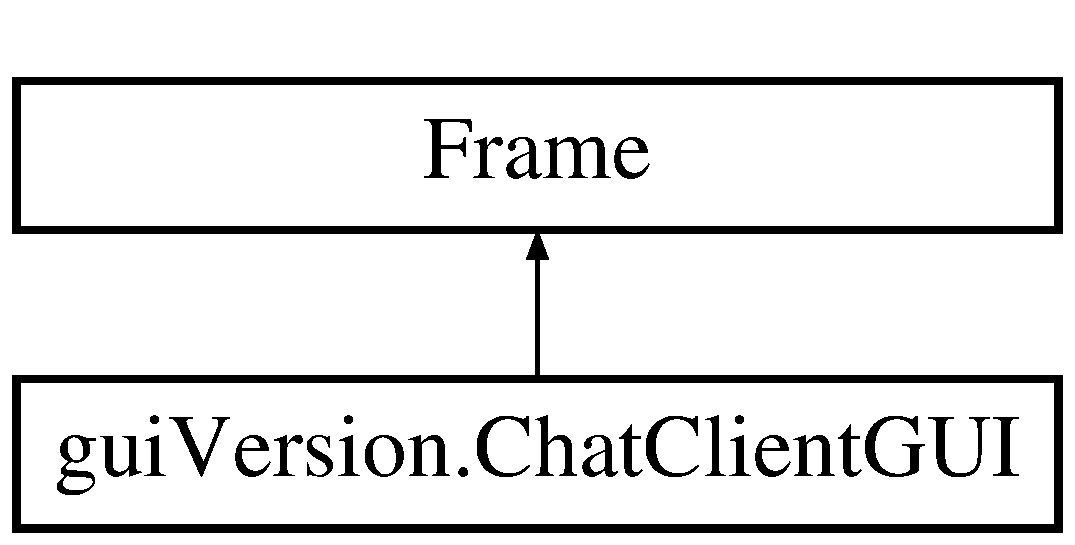
\includegraphics[height=2.000000cm]{class_frame}
\end{center}
\end{figure}


The documentation for this class was generated from the following file\+:\begin{DoxyCompactItemize}
\item 
\hyperlink{gui_version_8py}{gui\+Version.\+py}\end{DoxyCompactItemize}

\chapter{File Documentation}
\hypertarget{gui_version_8py}{}\section{gui\+Version.\+py File Reference}
\label{gui_version_8py}\index{gui\+Version.\+py@{gui\+Version.\+py}}
\subsection*{Classes}
\begin{DoxyCompactItemize}
\item 
class \hyperlink{classgui_version_1_1_f}{gui\+Version.\+F}
\item 
class \hyperlink{classgui_version_1_1_chat_client_g_u_i}{gui\+Version.\+Chat\+Client\+G\+U\+I}
\end{DoxyCompactItemize}
\subsection*{Namespaces}
\begin{DoxyCompactItemize}
\item 
 \hyperlink{namespacegui_version}{gui\+Version}
\end{DoxyCompactItemize}
\subsection*{Functions}
\begin{DoxyCompactItemize}
\item 
def \hyperlink{namespacegui_version_ae8a9c77879e18f58a45597b28e21042b}{gui\+Version.\+zip\+\_\+and\+\_\+encrypt\+\_\+val} (clear\+\_\+text, key)
\item 
def \hyperlink{namespacegui_version_a2925a99a40df97be6ae16f1a22184b24}{gui\+Version.\+decrypt\+\_\+val\+\_\+and\+\_\+unzip} (cipher\+\_\+text, key)
\item 
def \hyperlink{namespacegui_version_a79d3b927a5ac9c40a255afc12ebfa5bb}{gui\+Version.\+main} ()
\end{DoxyCompactItemize}
\subsection*{Variables}
\begin{DoxyCompactItemize}
\item 
tuple \hyperlink{namespacegui_version_ad80b491a9fbc91c221e73a124bff5d05}{gui\+Version.\+M\+A\+S\+T\+E\+R\+\_\+\+K\+E\+Y} = hashlib.\+sha256(\char`\"{}Some-\/long-\/base-\/key-\/to-\/use-\/as-\/encyrption-\/key\char`\"{})
\begin{DoxyCompactList}\small\item\em somethings wrong when the message number of characters!!! \end{DoxyCompactList}\item 
\hyperlink{namespacegui_version_a77c635f5f5d51002c89931af7228063c}{gui\+Version.\+old\+\_\+f} = sys.\+stdout
\end{DoxyCompactItemize}

\hypertarget{new_server_8py}{}\section{new\+Server.\+py File Reference}
\label{new_server_8py}\index{new\+Server.\+py@{new\+Server.\+py}}
\subsection*{Classes}
\begin{DoxyCompactItemize}
\item 
class \hyperlink{classnew_server_1_1_f}{new\+Server.\+F}
\end{DoxyCompactItemize}
\subsection*{Namespaces}
\begin{DoxyCompactItemize}
\item 
 \hyperlink{namespacenew_server}{new\+Server}
\end{DoxyCompactItemize}
\subsection*{Functions}
\begin{DoxyCompactItemize}
\item 
def \hyperlink{namespacenew_server_ae9d433fa51d0c682b18c3b9879cb0a1f}{new\+Server.\+process\+Client\+Commands} (cmd, client\+Socket)
\item 
def \hyperlink{namespacenew_server_a35090b3a9dc30b6f28f73efc7e104cc9}{new\+Server.\+send\+Response\+From\+Server} (response, user\+Socket)
\item 
def \hyperlink{namespacenew_server_af9cb120a81a10188d82dd3aaec0eea2d}{new\+Server.\+client\+Message} (client\+Soc, client\+Addr, server\+Socket)
\item 
def \hyperlink{namespacenew_server_a32d38e8c1989792b3d964150ed181779}{new\+Server.\+broadcast} (server\+\_\+socket, sock, message)
\item 
def \hyperlink{namespacenew_server_abe65059086c03efc53e029abe9cc98fc}{new\+Server.\+chat\+\_\+server} (host, port)
\end{DoxyCompactItemize}
\subsection*{Variables}
\begin{DoxyCompactItemize}
\item 
list \hyperlink{namespacenew_server_a85c087d4ca25a1782111a4dca1169b6d}{new\+Server.\+P\+O\+S\+S\+I\+B\+L\+E\+\_\+\+C\+O\+M\+M\+A\+N\+D\+S} = \mbox{[}\char`\"{}join\char`\"{},\char`\"{}bye\char`\"{},\char`\"{}crea\char`\"{},\char`\"{}subs\char`\"{},\char`\"{}unsu\char`\"{},\char`\"{}defa\char`\"{},\char`\"{}lscr\char`\"{},\char`\"{}lssu\char`\"{},\char`\"{}read\char`\"{},\char`\"{}writ\char`\"{},\char`\"{}chmod\char`\"{}\mbox{]}
\item 
string \hyperlink{namespacenew_server_a6c675879b0fb0559c66f1bf7118300fd}{new\+Server.\+H\+O\+S\+T} = '0.\+0.\+0.\+0'
\item 
list \hyperlink{namespacenew_server_a0472f2f3fb3afb95020b3c9ea29c0af4}{new\+Server.\+S\+O\+C\+K\+E\+T\+\_\+\+L\+I\+S\+T} = \mbox{[}$\,$\mbox{]}
\item 
int \hyperlink{namespacenew_server_a7d87ef1942af615eeec258c226e5b859}{new\+Server.\+R\+E\+C\+V\+\_\+\+B\+U\+F\+F\+E\+R} = 4096
\item 
int \hyperlink{namespacenew_server_a10c03320240322f838e9f19a686e825d}{new\+Server.\+P\+O\+R\+T} = 8022
\item 
\hyperlink{namespacenew_server_a771dfc755950f86e03d334f4d04dc59e}{new\+Server.\+old\+\_\+f} = sys.\+stdout
\end{DoxyCompactItemize}

%--- End generated contents ---

% Index
\backmatter
\newpage
\phantomsection
\clearemptydoublepage
\addcontentsline{toc}{chapter}{Index}
\printindex

\end{document}
